\documentclass[a4paper,12pt]{article}

\author{}
\date{}
\title{Filtration of ideal gas and \(C_5 H_{12}\)}

\usepackage[margin=0.9in]{geometry}
\usepackage{graphicx}
\usepackage{float}
\usepackage{textcomp}
\usepackage{amsmath, amssymb}
\usepackage{siunitx}
\usepackage{subcaption}
\usepackage{multirow}
\usepackage{bm}

\begin{document}
\maketitle
\section{The Physics}
We simulate 2d flow of ideal gas and \(C_5H_{12}\) through a
porous medium with the help of Darcy's law:
\begin{equation}
    \bm{v}_i = \frac{1}{\mu} \hat K \cdot f(s) \cdot 
    \nabla P
\end{equation}
where \(\hat K\), the specific permeability.
It depends only on the geometry of the medium.
We assume isotropy of space, so K is a scalar.
\(\mu\) is the dynamic viscosity.

As an approximation, \(f(s) = s^2\) for the first 
component, and \(f(s) = (1 - s)^2\) for the second.

The continuity equation for each component becomes:
\begin{equation}
    \varphi \frac{\partial \rho_i}{\partial t}
    + div (\rho_i \bm{v}_i) = 0
\end{equation}
where \(\rho_i = \frac{m_i}{V}\).

We use the Tait equation to relate liquid density to pressure:
\begin{equation}
    \frac{\rho - \rho_0}{\rho} = C \log_{10}
    \frac{B + P}{B + P_0}
\end{equation}
where \(C = 0.2105\),
\(\rho_0 = \frac{1}{67.28 \frac{m^3}{mol}}\),
\(P_0 = 0.1 MPa\), \(B = 35MPa\),
in the case of \(C_5H_{12}\).

Ideal gas equation of state:
\begin{equation}
    P = \frac{RT}{\mu}\rho
\end{equation}

\section{Boundary Conditions}

\begin{figure}[H]
    \centering
    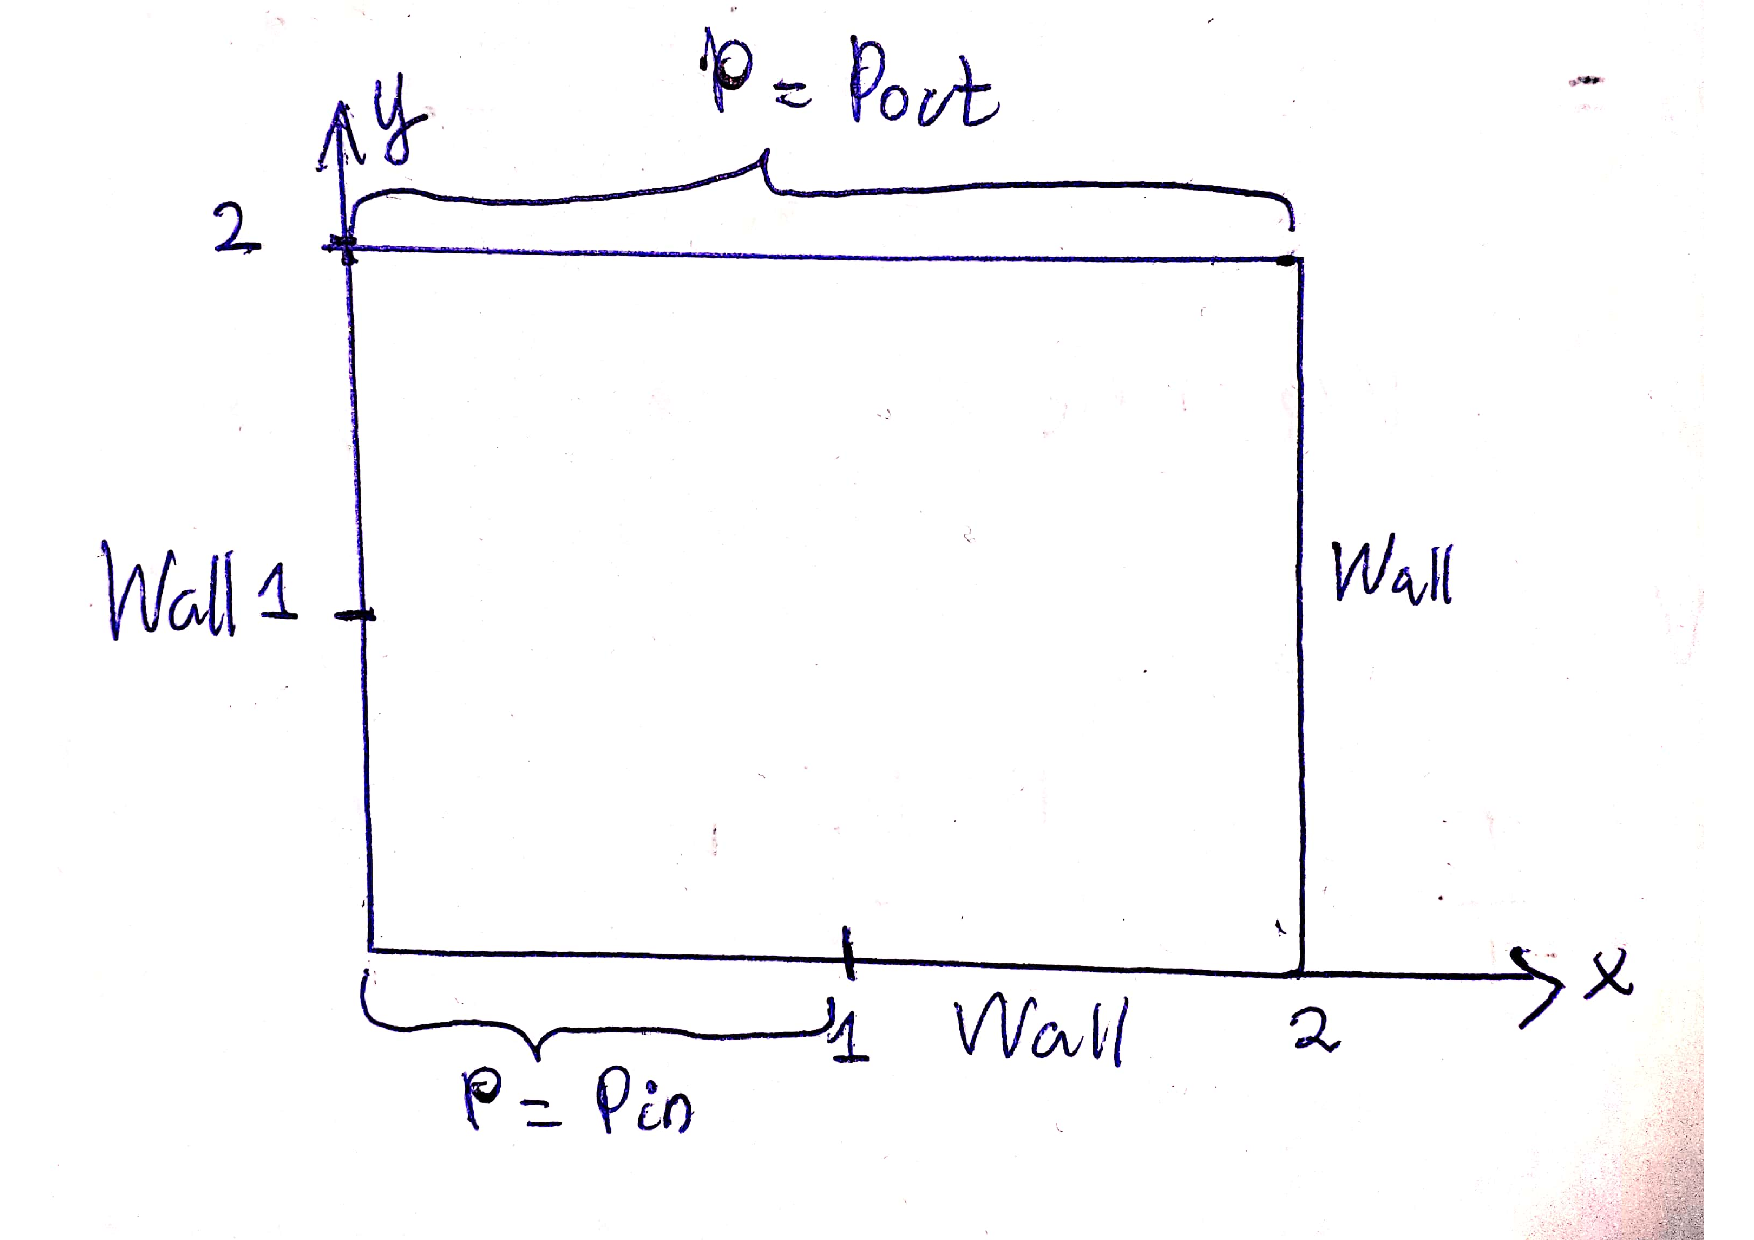
\includegraphics[width=0.5\textwidth]{img/diagram.pdf}
    \caption{Boundary Conditions}
    \label{fig:img-diagram-pdf}
\end{figure}

On pressure:
\[
\begin{cases}
    P = P_{in} &\text{at } y = 0
    \text{ and } x \in [0, 1] \\
    P = P_{out} &\text{at } y = 2 \\
    \frac{\partial P}{\partial x} = 0 &\text{at }
    x = 0, 2 \\
    \frac{\partial P}{\partial y} = 0 &\text{at }
    y = 0 \text{ and } x \in [1, 2]
\end{cases}
\] 

On velocities:
\[
\begin{cases}
    u = 0 &\text{at } x = 0, 2 \\
    v = 0 &\text{at } y = 0 \text{ and } x \in [1, 2] \\
    \frac{\partial v}{\partial y} = 0 &\text{at } y = 2 \\
    \frac{\partial v}{\partial y} = 0 &\text{at } y = 0
    \text{ and } x \in [0, 1]\\
\end{cases}
\] 

On density - ? 

On saturation - ?

\section{Algorithm}

Euler method for discretization with respect to time.
(TODO: upgrade to predictor-corrector).

Second order scheme in space, with the use of ghost cells. 

\begin{enumerate}
    \item Calculate densities for each component using EOS.
    \item Find the pressure and saturation with the
        help of binary search.
    \item Use Darcy's law to calculate velocities.
\end{enumerate}

% \section{TODO}
% \begin{enumerate}
%     \item Fix: \(\mu\) is different for each component.
%     \item Add boundary conditions on \(s_{n + 1} = s_n\)
%         in the borders.
% \end{enumerate}
\end{document}
